\title{Assignment 1: CS 663, Fall 2024}
\author{}
\date{Due: 23rd August before 11:55 pm}

\documentclass[11pt]{article}

\usepackage{amsmath}
\usepackage{amssymb}
\usepackage{hyperref}
\usepackage{ulem,graphicx}
\usepackage[margin=0.5in]{geometry}
\begin{document}
\maketitle

\textbf{Remember the honor code while submitting this (and every other) assignment. You may discuss broad ideas with other students or ask me for any difficulties, but the code you implement and the answers you write must be your own. We will adopt a \textbf{zero-tolerance policy} against any violation.}
\\
\\
\textbf{Submission instructions:} Follow the instructions for the submission format and the naming convention of your files from the submission guidelines file in the homework folder. Please see \textsf{assignment1.zip} in the homework folder. For all the questions, write your answers and scan them, or type them out in word/Latex. In eithe case, create a separate PDF file. The last two questions will also have code in addition to the PDF file. Once you have finished the solutions to all questions, prepare a single zip file and upload the file on moodle \emph{before} 11:55 pm on 23rd August.  We will not penalize submission of the files till 10 am on 24th August. \textbf{No assignments will be accepted after this time.} Please preserve a copy of all your work until the end of the semester.  \textbf{Your zip file should have the following naming convention:} RollNumber1\_RollNumber2\_RollNumber3.zip for three-member groups, RollNumber1\_RollNumber2.zip for two-member groups and RollNumber1.zip for single-member groups. 

\begin{enumerate}
\item Consider that you want to align two XRay images of a patient's forearm bone, one taken with pixel size $0.5 \times 0.5$ and the other with pixel size $0.25 \times 0.25$, using a control point based approach.  What motion model will you adopt to solve this problem and why? Now consider that the second image had a pixel size of $0.25 \times 0.5$. What motion model will you adopt to solve this problem and why? In both cases, do not use unnecessarily complicated motion models than what is required for the task at hand. All dimensions are in millimetres. \textsf{[5+5 = 10 points]}

\item A student is trying to align three images $I_1, I_2, I_3$. Let us assume that they are related to each other by purely translational motion. Let the motion from image $I_i$ to $I_j$ be denoted by $\boldsymbol{u_{ij}} \in \mathbb{R}^2$ where $i,j \in \{1,2,3\}, i \neq j$. What is the relationship between $\boldsymbol{u_{12}}, \boldsymbol{u_{23}}, \boldsymbol{u_{13}}$? When you perform motion estimation in practice, will that relationship hold in practice? Why (not)? There is no need to write any code for this. \textsf{[10 points]}

\item You are viewing the graph in Fig. 1 from a research paper. Unfortunately from the graph, the $(x,y)$ values at only a few points can be observed. You need to obtain the $(x,y)$ values at many other points. Hence you can do the following: you extract the image from the paper, and open it through MATLAB which provides a function called impixelinfo. This function gives you the $(x,y)$ coordinates of any spatial location pointed by your mouse. However, the coordinate system of the graph and that of MATLAB will be different. Describe a procedure to convert the coordinates of any point from MATLAB's coordinate system to the coordinate system of the graph. This will help you obtain the $(x,y)$ coordinates in the coordinate system of the graph. Support your answer with suitable equations. There is no need to write any code for this. 
\begin{figure}
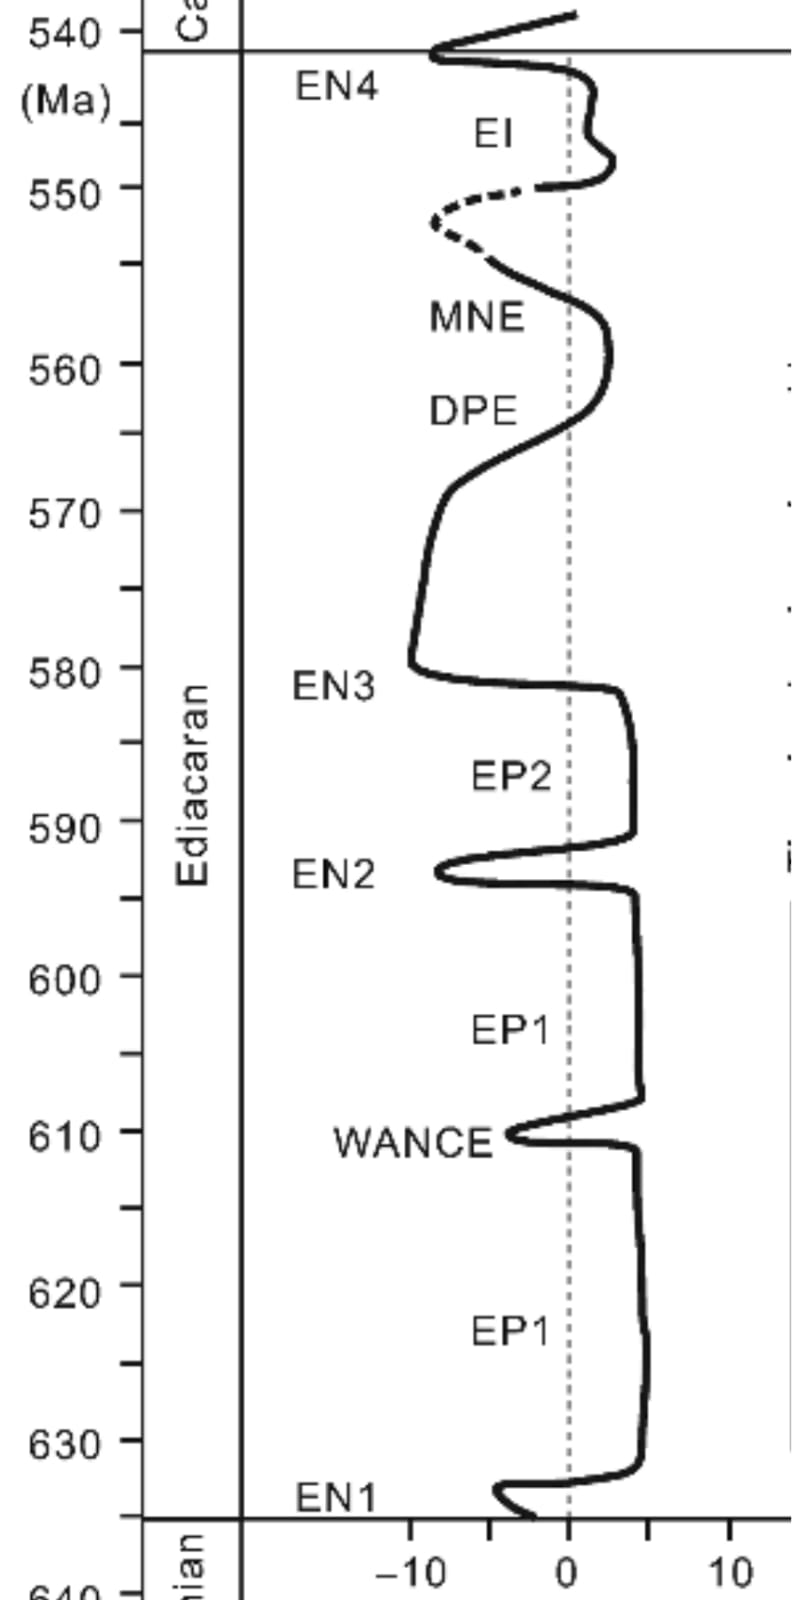
\includegraphics[scale=0.15]{graph.jpeg}
\label{fig:graph1}
\caption{Graph used for question 2.}
\end{figure}
\textsf{[15 points]}


\item Suppose the motion model between two images is expressed as follows: For any pair of physically corresponding points $(x_1,y_1)$ in image 1 and $(x_2, y_2)$ in image 2, we have: $x_2 = ax^2_1 + by^2_1 + c x_1 y_1 + d x_1 + e y_1 + f, y_2 = Ax^2_1 + By^2_1 + C x_1 y_1 + D x_1 + E y_1 + F$ where $a,b,c,d,e,f,A,B,C,D,E,F$ are all (unknown) constants. Explain how you will perform motion estimation using control points. Write down all key equations and the solution in the form of matrices and vectors. There is no need to write any code for this.
\textsf{[15 points]}

\item Read in the images T1.jpg and T2.jpg from the homework folder using the MATLAB function \texttt{imread} and cast them as a double array. Let us call these images as J1 and J2. These are magnetic resonance images of a portion of the human brain, acquired with different settings of the MRI machine. They both represent the same anatomical structures and are perfectly aligned (i.e. any pixel at location $(x,y)$ in both images represents the exact same physical entity). We are going to perform a simulation experiment for image alignment in a setting where the image intensities of physically corresponding pixels are different. To this end, do as follows:
\begin{enumerate}
\item Write a piece of MATLAB code to rotate the second image by $\theta = 28.5$ degrees anti-clockwise. You can use the \texttt{imrotate} function in MATLAB to implement the rotation using any interpolation method. Note that the rotation is performed implicitly about the centroid of the image. While doing so, assign a value of 0 to unoccupied pixels. Let us denote the rotated version of J2 as J3. 
\item Our job will now be to align J3 with J1 keeping J1 fixed. To this end, we will do a brute-force search over $\theta$ ranging from -45 to +45 degrees in steps of 1 degree. For each $\theta$, apply the rotation to J3 to create an intermediate image J4, and compute the following measures of dependence between J1 and J4:
\begin{itemize}
\item the normalized cross-correlation (NCC)
\item the joint entropy (JE)
\item a measure of dependence called quadratic mutual information (QMI) defined as $\sum_{i_1}\sum_{i_2} (p_{I_1 I_2}(i_1,i_2)-p_{I_1}(i_1)p_{I_2}(i_2))^2$, where $p_{I_1 I_2}(i_1,i_2)$ represents the \emph{normalized} joint histogram (\textit{i.e.}, joint pmf) of $I_1$ and $I_2$ (`normalized' means that the entries sum up to one). Here, the random variables $I_1, I_2$ denote the pixel intensities from the two images respectively. For computing the joint histogram, use a bin-width of 10 in both $I_1$ and $I_2$. For computing the marginal histograms $p_{I_1}$ and $p_{I_2}$, you need to integrate the joint histogram along one of the two directions respectively. You should write your own joint histogram routine in MATLAB - do not use any inbuilt functions for it. 
\end{itemize}
\item Plot separate graphs of the values of NCC, JE, QMI versus $\theta$ and include them in the report PDF. 
\item Determine the optimal rotation between J3 and J1 using each of these three measures. What do you observe from the plots with regard to estimating the rotation? Explain in the report PDF. 
\item For the optimal rotation using JE, plot the joint histogram between J1 and J4 using the \texttt{imagesc} function in MATLAB along with \texttt{colorbar}. Include it in the report PDF.
\item We have studied NCC and JE in class. What is the intuition regarding QMI? Explain in the report PDF. (Hint: When would random variables $I_1$ and $I_2$ be considered statistically independent?) 
 \textsf{[2+10+2+3+3+5=25 points]}
\end{enumerate}

\item Read in the images `goi1.jpg' and `goi2.jpg' from the homework folder using the MATLAB \texttt{imread} function and cast them as double. These are images of the Gateway of India acquired from two different viewpoints. As such, no motion model we have studied in class is really adequate for representing the motion between these images, but it turns out that an affine model is a reasonably good approximation, and you will see this. We will estimate the affine transformation between these two images in the following manner:
\begin{enumerate}
\item Display both images using \texttt{imshow(im1)} and \texttt{imshow(im2)} in MATLAB. Use the \texttt{ginput} function of MATLAB to manually select (via an easy graphical user interface) and store $n = 12$ pairs of physically corresponding salient feature points from both the images. For this, you can do the following: \\
\texttt{for i=1:12, figure(1); imshow(im1/255); [x1(i), y1(i)] = ginput(1); \\ figure(2); imshow(im2/255); [x2(i), y2(i)] = ginput(1);}\\
\textbf{Tips:} Avoid selecting points which are visible in only one image. Try to select them as accurately as possible, but our procedure is robust to small sub-pixel errors. Make sure \texttt{x1(i),y1(i)} and \texttt{x2(i),y2(i)} are actually physically corresponding points. Salient feature points are typically points that represent corners of various structures. 
\item Write MATLAB code to determine the affine transformation which converts the first image (`goi1') into the second one (`goi2'). 
\item Using nearest neighbor interpolation that you should implement \emph{yourself}, warp the first image with the affine transformation matrix determined in the previous step, so that it is now better aligned with the second image. You are not allowed to use any implementation for this already available in MATLAB. Display all three images side by side in the report PDF.
\item Repeat the previous step with bilinear interpolation that you should implement \emph{yourself}. You are not allowed to use any implementation for this already available in MATLAB. Display all three images side by side in the report PDF.
\item In the first step, suppose that the $n$ points you chose in the first image happened to be collinear. Explain (in the report PDF) the effect on the estimation of the affine transformation matrix. 
\textsf{[5+5+5+5+5=25 points]}
\end{enumerate}


\end{enumerate}



\end{document}